\documentclass{jsarticle}
\usepackage[dvipdfmx]{graphicx}
\usepackage{amsmath}

\begin{document}
\thispagestyle{empty}
\begin{center}
\vspace*{4.5cm}
{\huge\bf cubing暗号の提案}
\vspace*{3cm}

{\large 20XX年X月提出日}
\vspace*{3cm}

{\large 立命館大学 情報理工学部}
\vspace*{5mm}

{\Large 石~川~~琉~聖}
\end{center}
\newpage 

\setcounter{page}{1}

\section*{概要}

研究論文の内容について、500 - 600 字程度でまとめる。
この概要を読めば、大体どういうことを研究したのかがわかるように書く。
具体的には、どういう問題について、どのような研究を行って、その結果どのような
結論が得られたか、というポイントについて簡潔にまとめる。

\newpage

\tableofcontents
\clearpage

\section{はじめに}
暗号がここらへんで使われててそこそこ大事って言う社会的背景を語る

\section{準備}
\subsection{記号の定義}
ここ要りますか.要らないかも.
\subsection{暗号化とは}
ここは「1.はじめに」に含んでも良さそう
先に下を書き,この用語の説明が必要と言ったものがあれば書く
もはやこの章要らなそう

\section{本論}
\subsection{cubing暗号の概要}
cubing暗号の概要は以下の通りである.
\begin{itemize}
  \item 平文ブロック長:45byte
  \item 暗号文ブロック長:108byte
  \item 鍵長:可変
  \item 暗号化処理の並列化:可 (※但し,Shuffle処理がボトルネックとなる)
  \item 復号処理の並列化:可 (※但し,Sort処理がボトルネックとなる)
  \item Random Read:不可
\end{itemize}
なお,cubing暗号は暗号利用モード「cubingmode(CBGモード)」の利用を前提とし,以下cubing暗号に対しcubingmodeを利用した際の手順を説明する.
\subsection{cubing暗号の暗号化・復号手順}

以下の順序で暗号化・復号を行う.

\subsubsection{暗号化}
\begin{enumerate}
\item 平文を用意する.
\item 必要があればパディング処理を行う.
\item encrypt処理を行う.
\end{enumerate}

\subsubsection{復号}
\begin{enumerate}
\item decrypt処理を行う.
\item パディング処理を逆に行う.つまり,暗号化の際に付属した文字を取り除く.
\item 平文を取得する.
\end{enumerate}

\subsubsection{パディング処理}
平文ブロックが45Byteに満たない場合,1Byte分null入れ,残りはランダムな英数列を入れる.これにより,平文を45Byteに固定することができる.

\subsubsection{コンピュータ上での表現方法}
ルービックキューブをコンピュータ上で表現する際には配列を用いる.具体的には以下のルービックキューブの展開図と配列の添字が対応する.\\

\begin{center}
  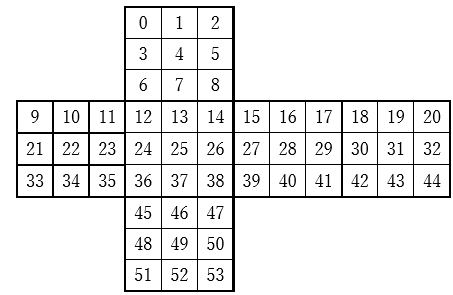
\includegraphics[width=7cm]{./tex_pic/seq.jpg}\\
\end{center}
    
\subsubsection{転置の仕様}
cubing暗号転置処理は方向・列・回数の三つより決定される.方向に関しては以下の図のように三種類定義される.縦方向はルービックキューブで処理する際,以下の図のように回転させる方向のことである.なお,図には各方向に対する列が記載されている.
\begin{center}
  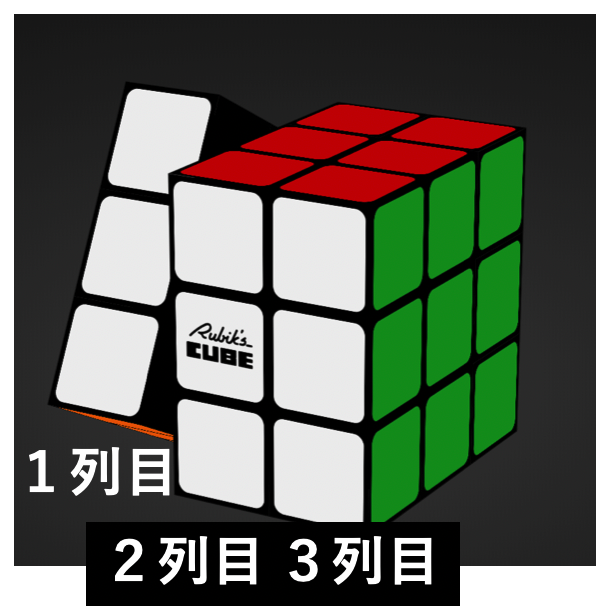
\includegraphics[width=7cm]{./tex_pic/tate.jpg}\\
\footnote{http://iamthecu.be/}
\end{center}
横方向に関しては以下のように定義されている.
\begin{center}
  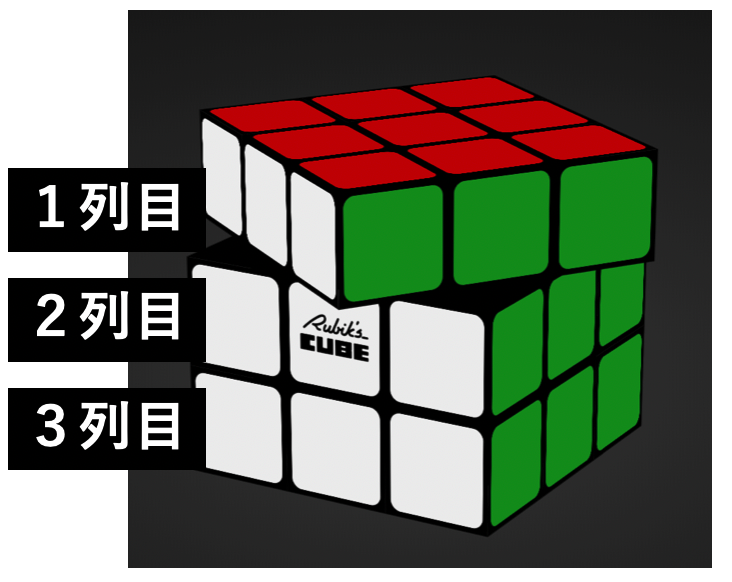
\includegraphics[width=7cm]{./tex_pic/yoko.jpg}\\
\footnotemark[1]
\end{center}
回転方向に関しては以下のように定義されている.
\begin{center}
  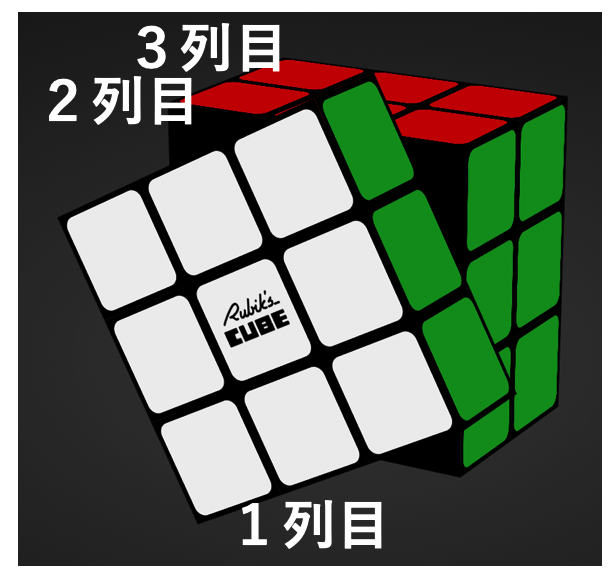
\includegraphics[width=7cm]{./tex_pic/kai.jpg}\\
\footnotemark[1]
\end{center}

なお,cubing暗号の転置はルービックキューブの転置とは一部違った箇所がある.それは,「ある方向のある列を転置させる際,他の列およびマスは一切転置させない」ということである.具体的には以下の図のような転置がなされる.\\
\\
\LARGE
\bf{暇な自分へ\\}
\normalsize
「1」「2」「3」\\
↓\\
「2」「3」「1」\\
みたいな図入れて\\

これにより,「ルービックキューブの角は常に同じ文字が隣り合っている」といった性質がなくなり,後述の頻度分析による解読の対策となる.


\subsubsection{暗号文の取得}
最後に,暗号文は以下の図の順で取り出す.
\begin{center}
  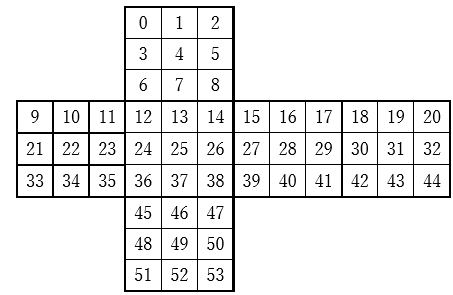
\includegraphics[width=7cm]{./tex_pic/seq.jpg}\\
\end{center}
\subsection{cubingmodeの利用手順}

以下の順序で暗号化・復号を行う.
\subsubsection{暗号化}
\begin{enumerate}
\item 平文をブロックに分ける.
\item 必要があればパディングを用意する.
\item 全ての平文に対してマスク処理を行う.
\item 全てのブロックに対し,エンコードを行う.
\item 全てのブロックの平文以外の箇所に対してマスク処理を行う.
\item ブロックごとに暗号化を行う.
\item ブロックをシャッフルする.
\end{enumerate}

\subsubsection{復号}
\begin{enumerate}
\item 暗号文をブロックに分ける.
\item 全てのブロックに対して復号を行う.
\item 暗号化の(5)で使用したマスク処理を元に戻す.
\item (3)により現れるシーケンス番号を元に,ブロック間ソートを行う.
\item 暗号化の(3)で使用したマスク処理を元に戻す.
\item 全てのブロックに対し,デコードを行う.
\item 全てのブロックを結合させ,平文を生成する.
\end{enumerate}

\subsubsection{cubingmodeの各処理の適用範囲}
各ブロックの内容は以下の通りである.また,mask(1)とmask(2)処理の適用範囲に関しても以下の通りである.
\begin{center}
  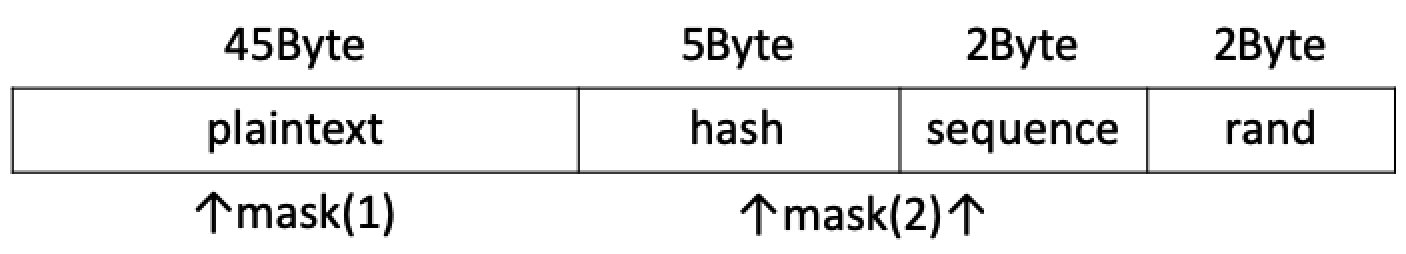
\includegraphics[width=12cm]{./tex_pic/block.png}\\
\end{center}

\subsubsection{62進数の説明}
cubingmodeのエンコード処理内では62進数が使われる.62進数は,「AA, AB, AC, ... , AZ, Aa, Ab, Ac, ... , A0, A1, A2, ... , A9, BA, BB, ... , B9, CA, ... , 99, ...」の順で定義される.なお,本暗号利用モードではAA~99までが使用される.

\subsubsection{エンコード処理}
本節では以下の記号を用いる.

\(n\):現在操作しているブロックの番号(0,1,2,...)\\
\(C_i\):ブロックの\(i\) Byte目の文字\\
\(\mathrm{toas}(C)\):特定の文字\(C\)のASCIIコードにおける番号\\
\(\mathrm{fras}(N)\):特定の数字\(N\)のASCIIコードにおける文字\\
\(\mathrm{rand}()\):アルファベット又は数字から1文字を一様に選ぶ関数\\
\(\mathrm{to62}(x)\):0から61までの自然数xを62進数に従って文字にする関数

\begin{align}
C_{45+i} &= \mathrm{fras}\left(\left(\left(\sum_{j=9(i-1)+1}^{9i}{\mathrm{toas}(C_j)}\right)\bmod 26\right)+97\right) \notag\\
C_{51} &= \mathrm{to62}\left (\left \lfloor\frac{n}{62}\right \rfloor \right) \notag\\
C_{52} &= \mathrm{to62}\left ( n \bmod 62 \right) \notag\\
C_{53} &= \mathrm{rand}() \notag\\
C_{54} &= \mathrm{rand}() \notag\\
\end{align}

とする.ただし,\(i=1,2,3,4,5\)とする.これを全てのブロックに対して行う.

\subsubsection{表示可能文字}
以下の配列で定義される.
\begin{verbatim}
printable_table[] = {'0', '1', '2', '3', '4', '5', '6', '7', '8', '9', 
'a', 'b', 'c', 'd', 'e', 'f', 'g', 'h', 'i', 'j', 'k', 'l', 'm', 'n', 'o',
'p', 'q', 'r', 's', 't', 'u', 'v', 'w', 'x', 'y', 'z', 'A', 'B', 'C', 'D',
'E', 'F', 'G', 'H', 'I', 'J', 'K', 'L', 'M', 'N', 'O', 'P', 'Q', 'R', 'S',
'T', 'U', 'V', 'W', 'X', 'Y', 'Z', '!', '"', '#', '$', '%', '&', '\'', '(',
')', '*', '+', ',', '-', '.', '/', ':', ';', '<', '=', '>', '?', '@', '[', 
'\\', ']', '^', '_', '`', '{', '|', '}', '~', ' ', '\n', '\0', '\t'};
\end{verbatim}

この順序はpythonのstring.printableを元に作られた.エスケープシーケンスに関してはASCIIコードに対応している.

\subsubsection{mask(1)処理}
mask(1)では各ブロックの平文45Byteにマスク処理を行う.まず,以下を定義する.\\
平文の\(i\)文字目:\(Pi\)\\
\(i\)番目のマスク:\(Mi\)\\
\(\mathrm{printable\_table}\)内の文字\(Pi\)のインデックス:\(\mathrm{Idx}(Pi)\) (※\(\mathrm{printable\_table}\)とは,上記「表示可能文字」のこと)\\
とすると,


\[Pi=\mathrm{printable\_table}[(\mathrm{Idx}(Pi)+Mi) \bmod 98]\\\]


と定義する.ただし,\(i=1〜45\)とする.

\subsubsection{mask(2)処理}
mask(2)ではハッシュとシーケンス番号にマスクをかける.計算方法は上記「mask(1)」と同様.

\subsubsection{encrypt処理}
encrypt処理ではcubing暗号の暗号化処置(転置処理)を行う.

\subsubsection{decrypt処理}
decrypt処理ではcubing暗号のencrypt処理を元に復号処理を行う.ルービックキューブは同じ方向・同じ列で4回回転させると元に戻る性質があるため,暗号化に回転した回数を\(n\)とおくと,復号処理では\(4-n\)回転置処理を行う.

\subsubsection{shuffle処理}
暗号化後に全ブロックをブロックごとにシャッフルする.Fisher–Yatesのアルゴリズムを用いることによって高速に実現可能となる.

\subsubsection{sort処理}
各ブロックの51,52番目の文字が昇順になるようにブロックごとにソートする.

\subsubsection{送信内容}
送信内容は以下の三つで構成され,三つが連結された状態で送信される.

1. 暗号文
2. mask(1)
3. mask(2)
ただし,mask(2)に関してはどのmask(2)がどのブロックに適用されるのか判別するため,各ブロックの後ろに記述する.
例) [block1] [mask(2)-1] [block3] [mask(2)-3] [block2] [mask(2)-2]

\subsubsection{ブロック数が多い時の対策}
\(62^2\)のブロックを1つの大きなブロックとして考え,各大きなブロックをECBモードで暗号化する.
上記「shuffle」では,\(62^2\)個の大きなブロックごとにシャッフルする.

\section{評価実験}
ここでは主に本暗号・暗号利用モードの長所を実験結果をもとに記す.
\subsection{推奨する鍵の長さに関して}
鍵の長さを変えた時,転置されている割合を計算\\
\subsubsection{数学的アプローチ}
\LARGE
\bf{---怪しい理論入ります---\\}
\normalsize
1回の転置処理で12/54文字変化する.つまり,1回の転置処理で42/54文字は変化しない.\\
ここで$n=$転置処理の回数とする.すると,特定の文字が変化しない確率は
\[\left(\frac{42}{54}\right)^n\]
で計算できる.ここで,全ての文字の変化する確率と変化しない確率を等しくするためには(全ての文字のエントロピーを等しくするためには??),以下の式が成り立つ必要がある.
\[\left(\frac{42}{54}\right)^n \leq \frac{1}{54}\]

これを満たす最小の$n$は16で,この時の左辺の値は約0.0179である.また,鍵長$=$転置回数$\times 3$なので,鍵長は$16*3=48$文字以上を推奨する.

\subsubsection{機械的アプローチ}
\LARGE
\bf{後でやる\\}
\normalsize

\subsection{AES・RSAとの実行時間の比較}
具体的なやり方は考えておらず,おそらくOpenSSLなるものを活用することになる
\subsubsection{AESとの比較}
\subsubsection{RSAとの比較}

\subsection{攻撃対策}
\subsubsection{ブルートフォース攻撃}
ここは計算量示すだけ
\subsubsection{頻度分析}
これより下はできないことを証明する
\subsubsection{選択平文攻撃}
\subsubsection{replay攻撃}

\section{関連研究}
\subsection{関連研究1(仮)}
mitchel cryptsystem
\subsection{関連研究2(仮)}
\subsection{関連研究3(仮)}

\section{まとめ}
\subsection{まとめ1(仮)}
\subsection{まとめ2(仮)}
\subsection{まとめ3(仮)}
\section{謝辞}
どこまで書けばいいのだろう..?その時の気分??

\newpage 
%% 参考文献テンプレ
文献ですか.
・研究論文
・暗号利用モード関連
・RSA,AESらへん
・replay攻撃らへん
・選択平文攻撃・暗号化オラクルらへん
・ルービックキューブの全探索にかかる手数
・その他(?)

\begin{thebibliography}{}

\bibitem{長尾} 長尾真:知識と推論,岩波講座ソフトウェア科学14 (1988). 

\bibitem{実近} 実近憲昭: ゲームと AI,人工知能学会誌 vol.5, pp.527-537, 1990.

\end{thebibliography}

\end{document}
